\documentclass[twoside]{article}

\usepackage{amsmath}
\usepackage{amsfonts}
\usepackage{graphicx}
\usepackage{multirow}
\usepackage{fontspec}
\usepackage{hyperref}
\usepackage{xepersian}
% Font Settings ======================
\setlatintextfont{LinLibertine}[Path = fonts/latin/]
\settextfont{HMXKayhan}[
Path = fonts/fa/ ,
BoldFont = HMXKayhanBd]
% Graphic Settings ===================
\graphicspath{{images/}}
\DeclareGraphicsExtensions{.jpeg,.png,.jpg}


\title{\Huge گزارش آزمایش 2 آز مدار منطقی }
\author{\Large علی دهقانی ، ماهان بیهقی}
\date{دانشگاه صنعتی شریف}

\begin{document}
	\maketitle
	\newpage
	\section*{نام آزمایش}
	مشخصه گیت NAND و آشنایی با مفهوم Fan-out
	
	\section*{اهداف آزمایش}
	آشنایی با مفهوم مشخصه انتقالی در مدارهای الکتریکی و پدیده Fan-out در تراشه های TTL
	
	\section*{شرح آزمایش}
	
	\subsection*{لیست تراشه ها و قطعات مورد نیاز}
	تراشه DM74LS00 , منبع تغذیه 5 ولت DC , مقاومت 1 کیلواهم , اسیلوسکوپ , پتانسیومتر
	
	\subsection*{مراحل آزمایش و مدارات}
	\begin{itemize}
		\item			
		یک منبع تغذیه متغیر میسازیم. برای اینکار از منبع تغذیه موجود 5 ولت و پتانسیومتر استفاده میکنیم. یک سر پتانسیومتر به زمین و سر دیگر به منبع dc متصل است. با تغییر مقدار مقاومت ، ولتاژ پایه سوم از 0 تا 5 تغییر میکند.
		
		\begin{figure}[h!]
			\begin{center}
				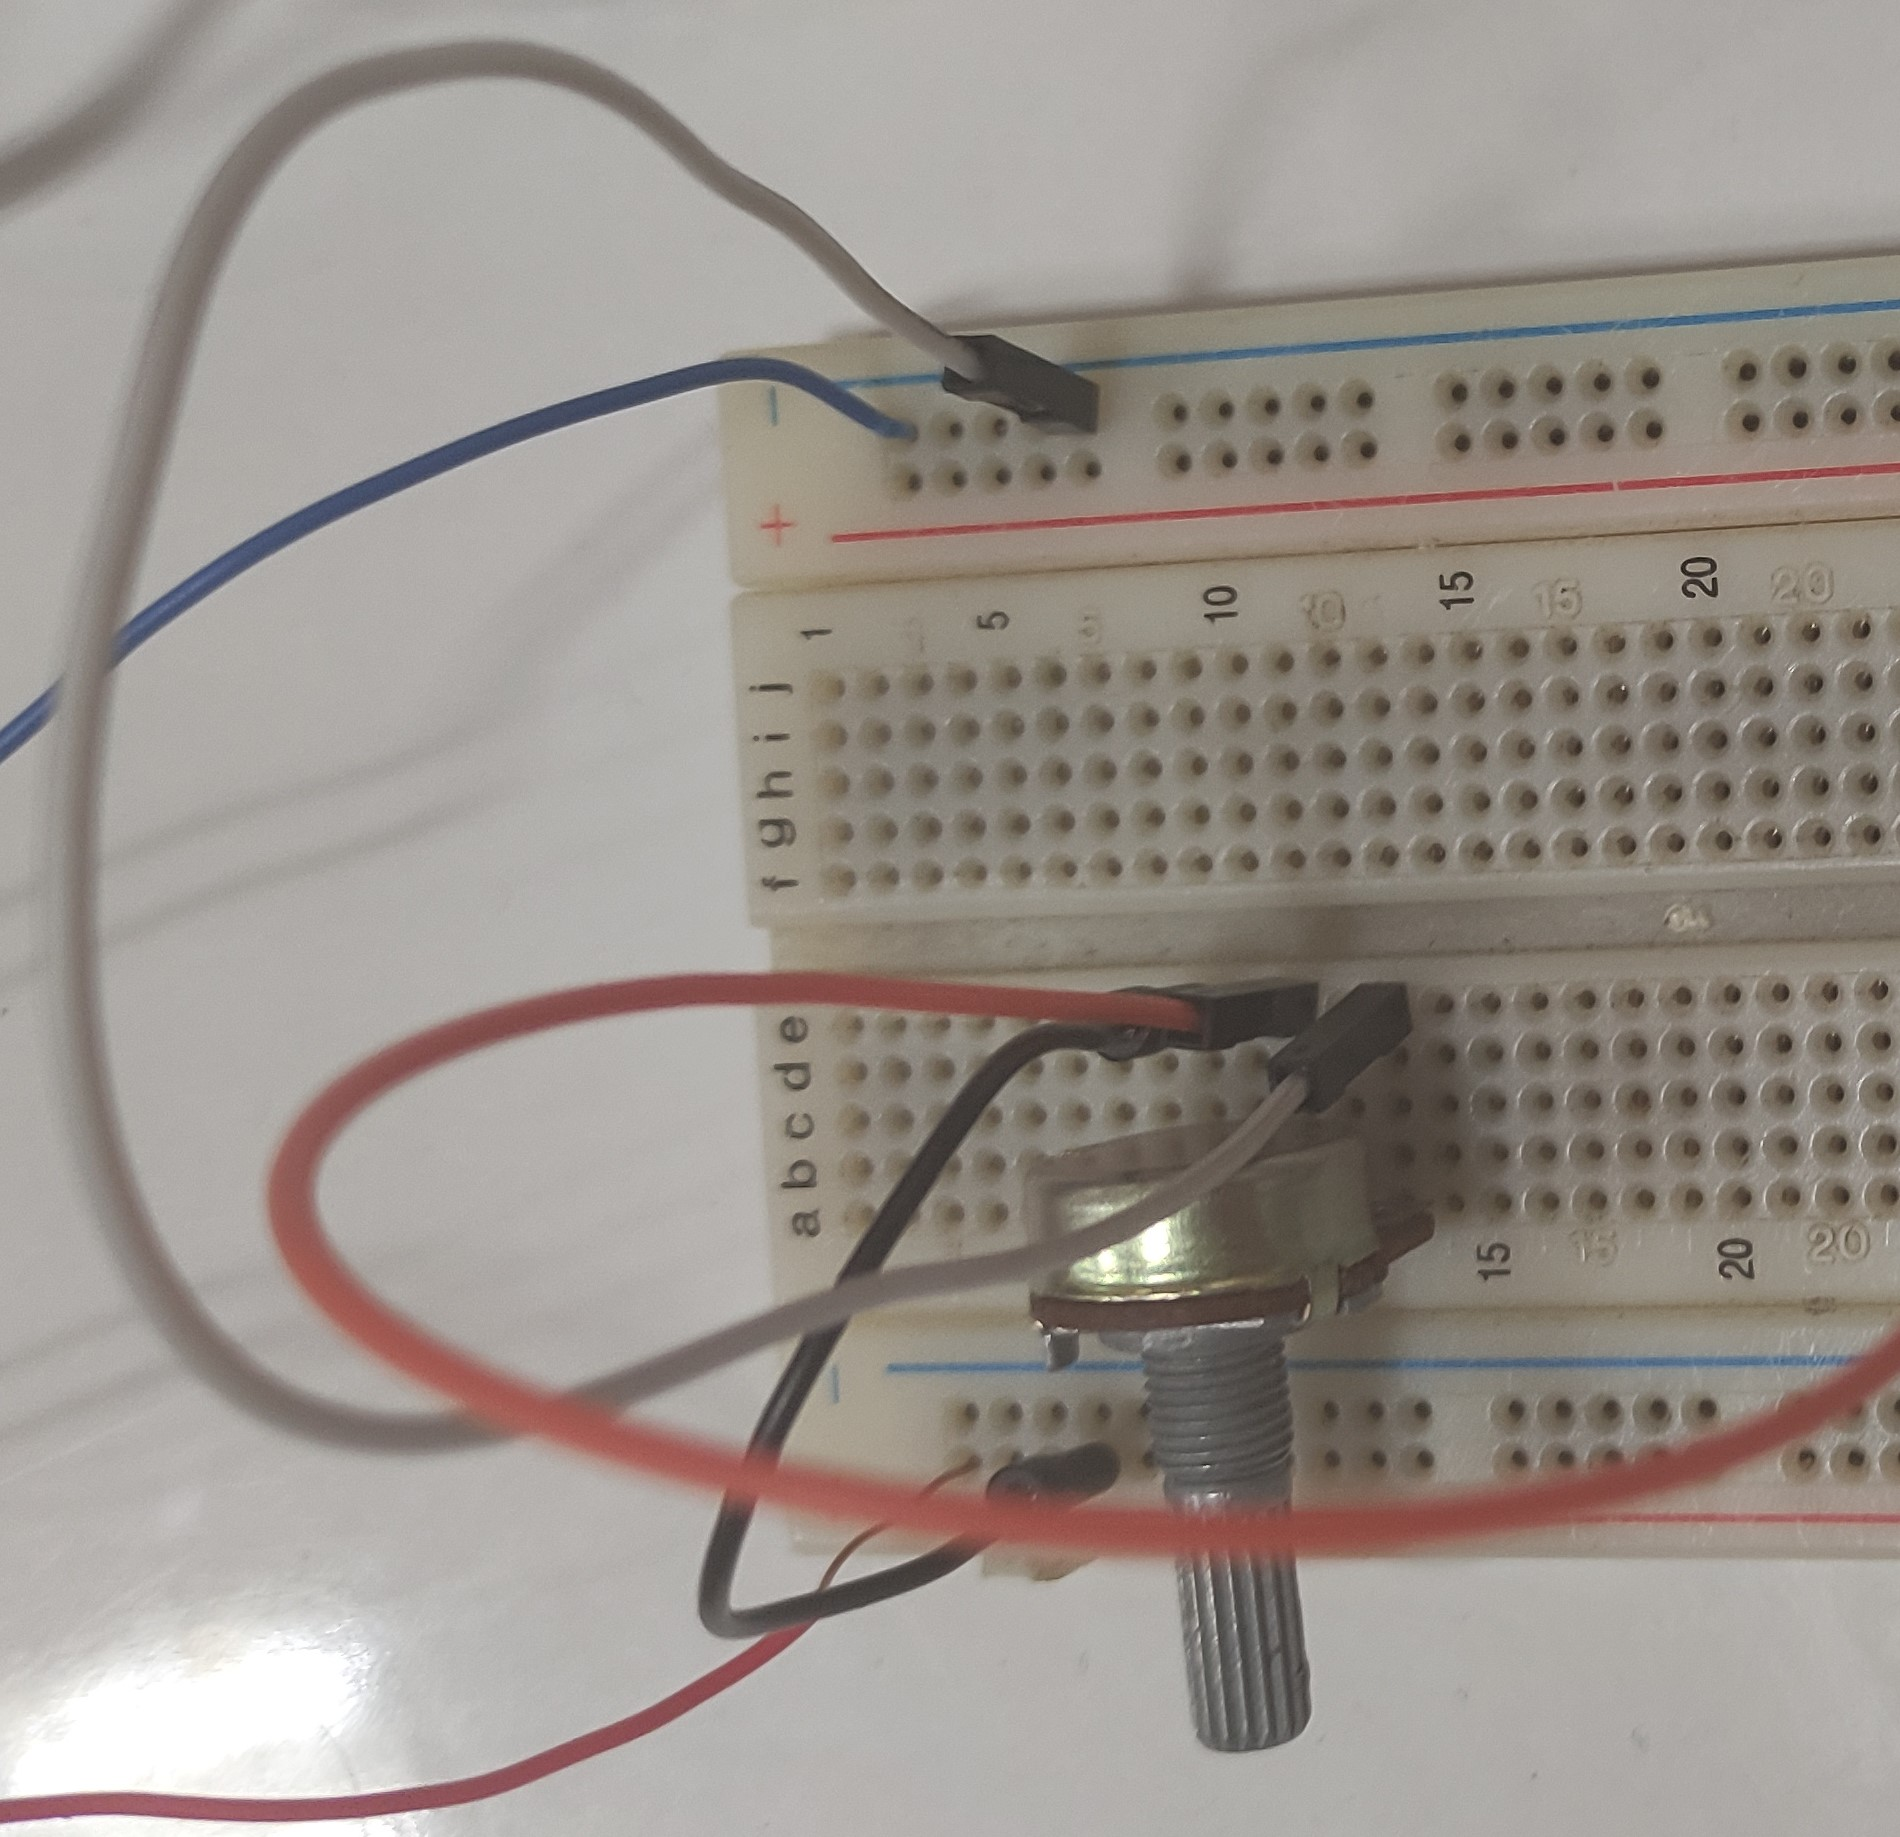
\includegraphics[scale=0.1]{variable_voltage_irl}‎
				\caption{منبع متغیر}
			\end{center}
		\end{figure} 
		
		\item			
		پایه A1 یک تراشه 7400 را به منبع ولتاژ متغیر و پایه B1 را به 5 ولت ثابت وصل میکنیم . خروجی این دو پایه مطابق دیتاشیت تراشه روی پایه Y1 خواهد بود. 
		
		\begin{figure}[h!]
			\begin{center}
				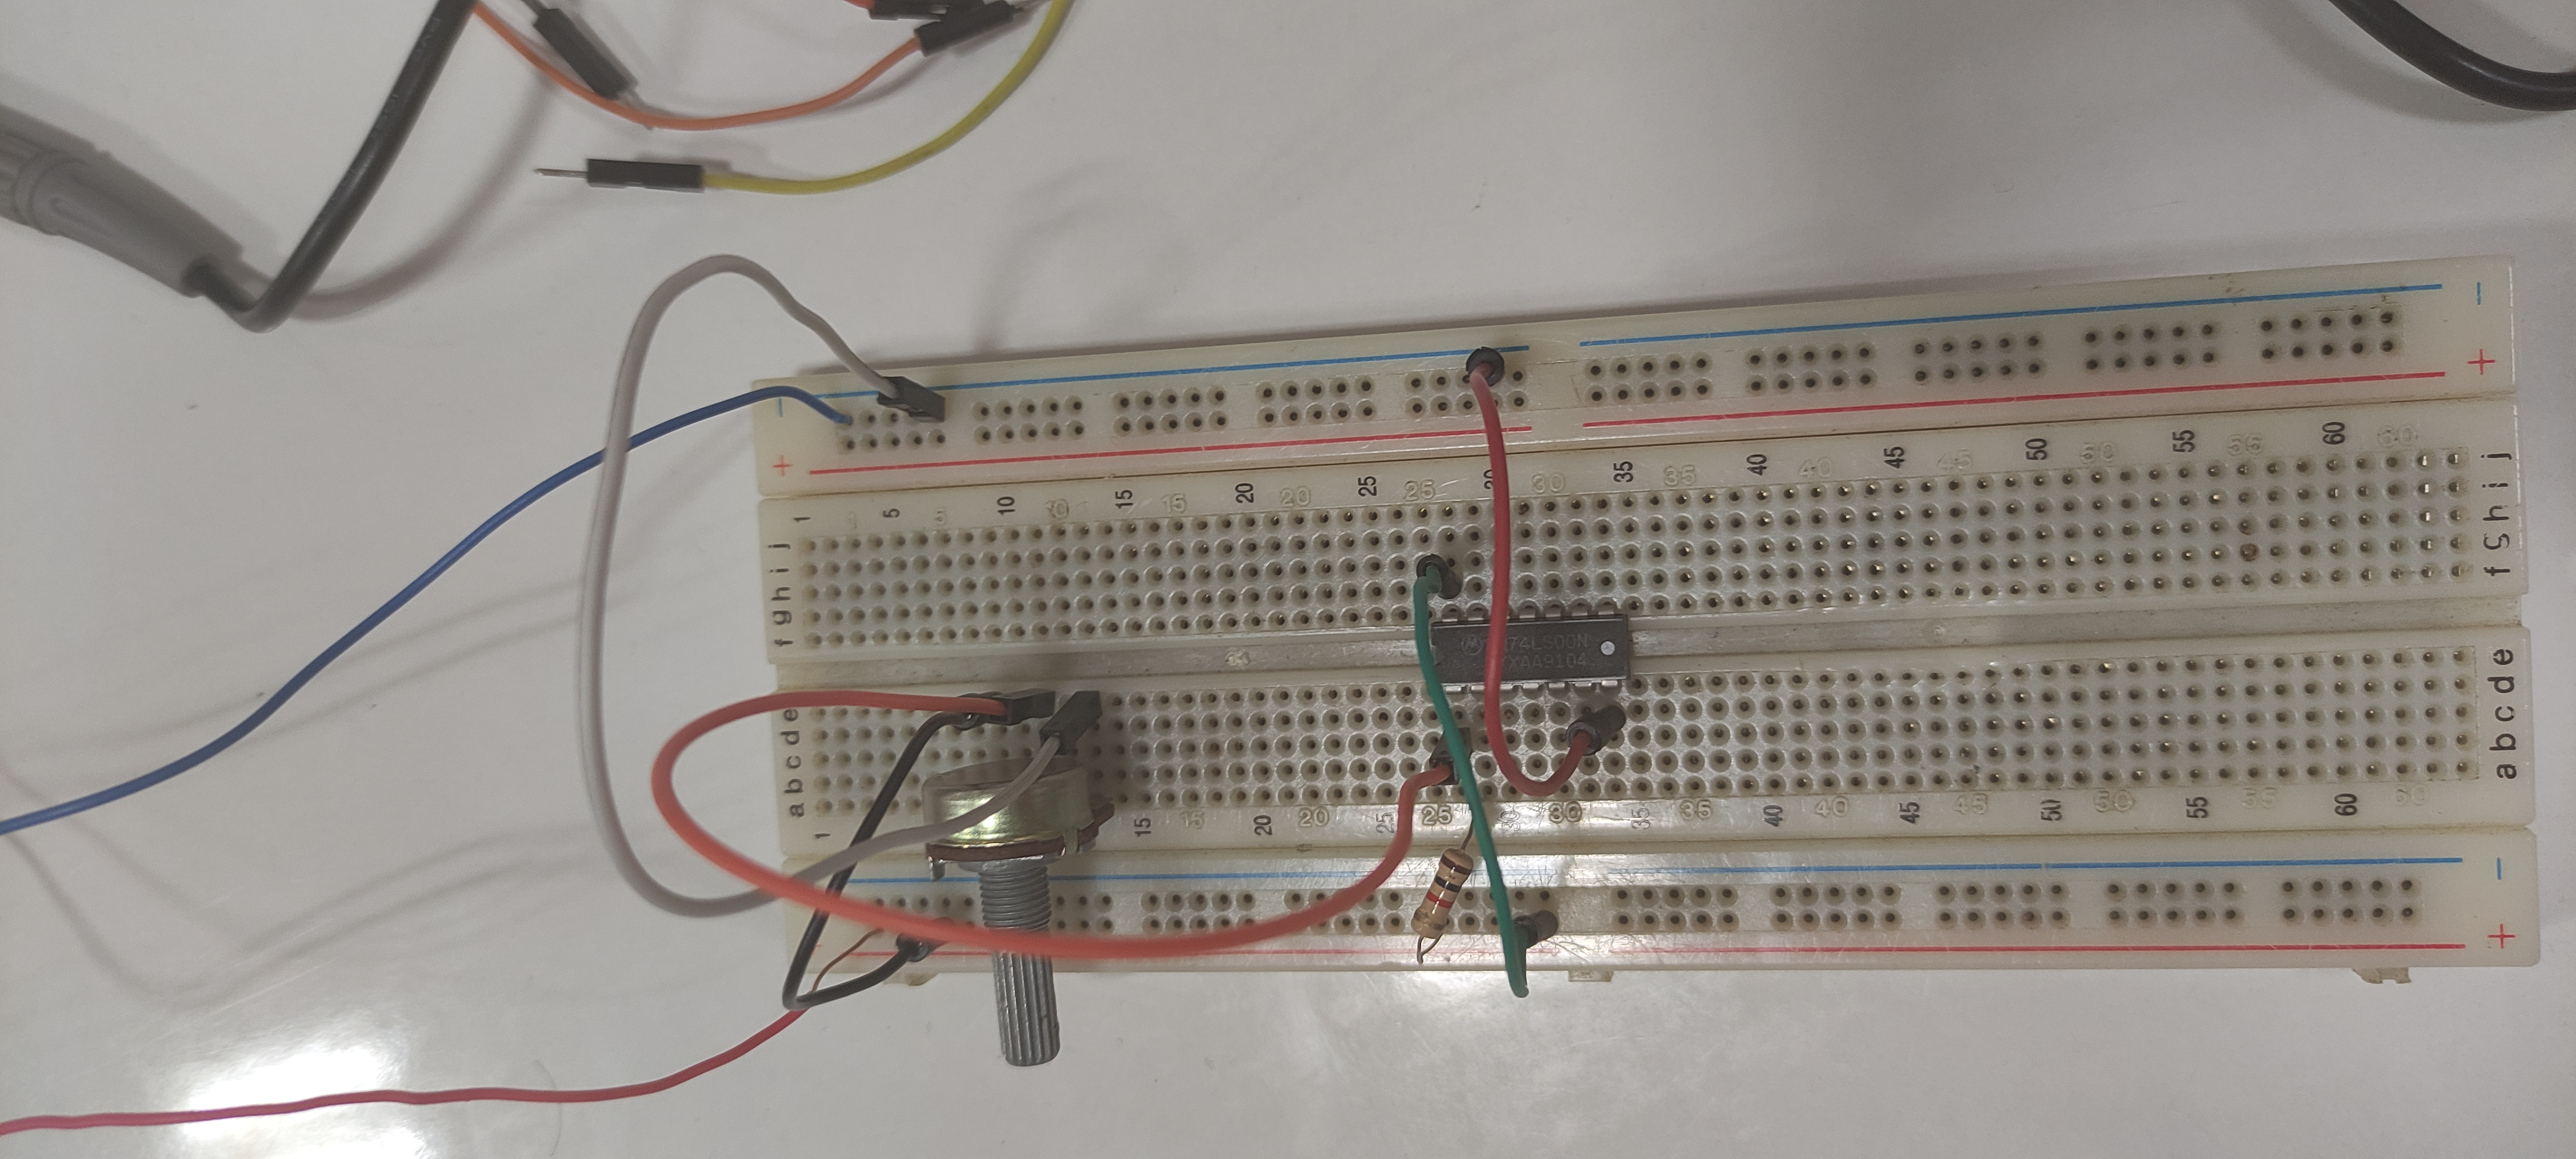
\includegraphics[scale=0.075]{first_madar_irl}‎
				\caption{مدار اندازه گیری ولتاژ پایه Y1 تراشه}
			\end{center}
		\end{figure} 
	
	\item
	در هر مرحله ولتاژ منبع متغیر را پنج دهم ولت تغییر میدهیم و ولتاژ خروجی پایه Y1 را اندازه گیری میکنیم. نمودار های به دست آمده در حالت های افزایش ولتاژ از 0 تا 5 و کاهش ولتاژ از 5 تا 0 مطابق زیر میشوند :
	\begin{figure}[h!]
		\begin{center}
			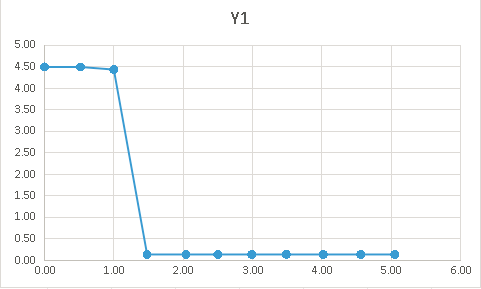
\includegraphics[scale=0.75]{nemoodar1}‎
			\caption{ولتاژ پایه Y1 در حالت نزولی}
		\end{center}
	\end{figure} 

	\begin{figure}[h!]
		\begin{center}
			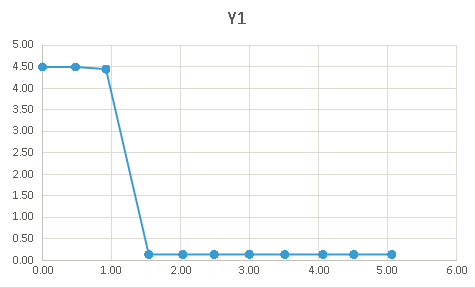
\includegraphics[scale=0.75]{nemoodar2}‎
			\caption{ولتاژ پایه Y1 در حالت صعودی}
		\end{center}
	\end{figure} 

		\newpage
		\item
		در مرحله بعد آزمایش خروجی گیت NAND را به ورودی های 10 گیت مشابه متصل میکنیم. برای اینکار از 3 تراشه مشابه استفاده میکنیم که vcc هر تراشه از gnd تراشه قبلی تغذیه میشود و تنها vcc تراشه اول و gnd تراشه سوم مستقل میباشند. انتظار میرود با افزایش تعداد گیت ها ، ولتاژ دچار افت شود. برای اندازه گیری این افت از پایه Y1 هر تراشه مقادیر ولتاژ خروجی رو در جدولی یادداشت میکنیم. نمودار های ولتاژ خروجی  از تراشه های 1 و 2 و 3 مطابق شکل های زیر میباشند :
		\begin{figure}[h!]
			\begin{center}
				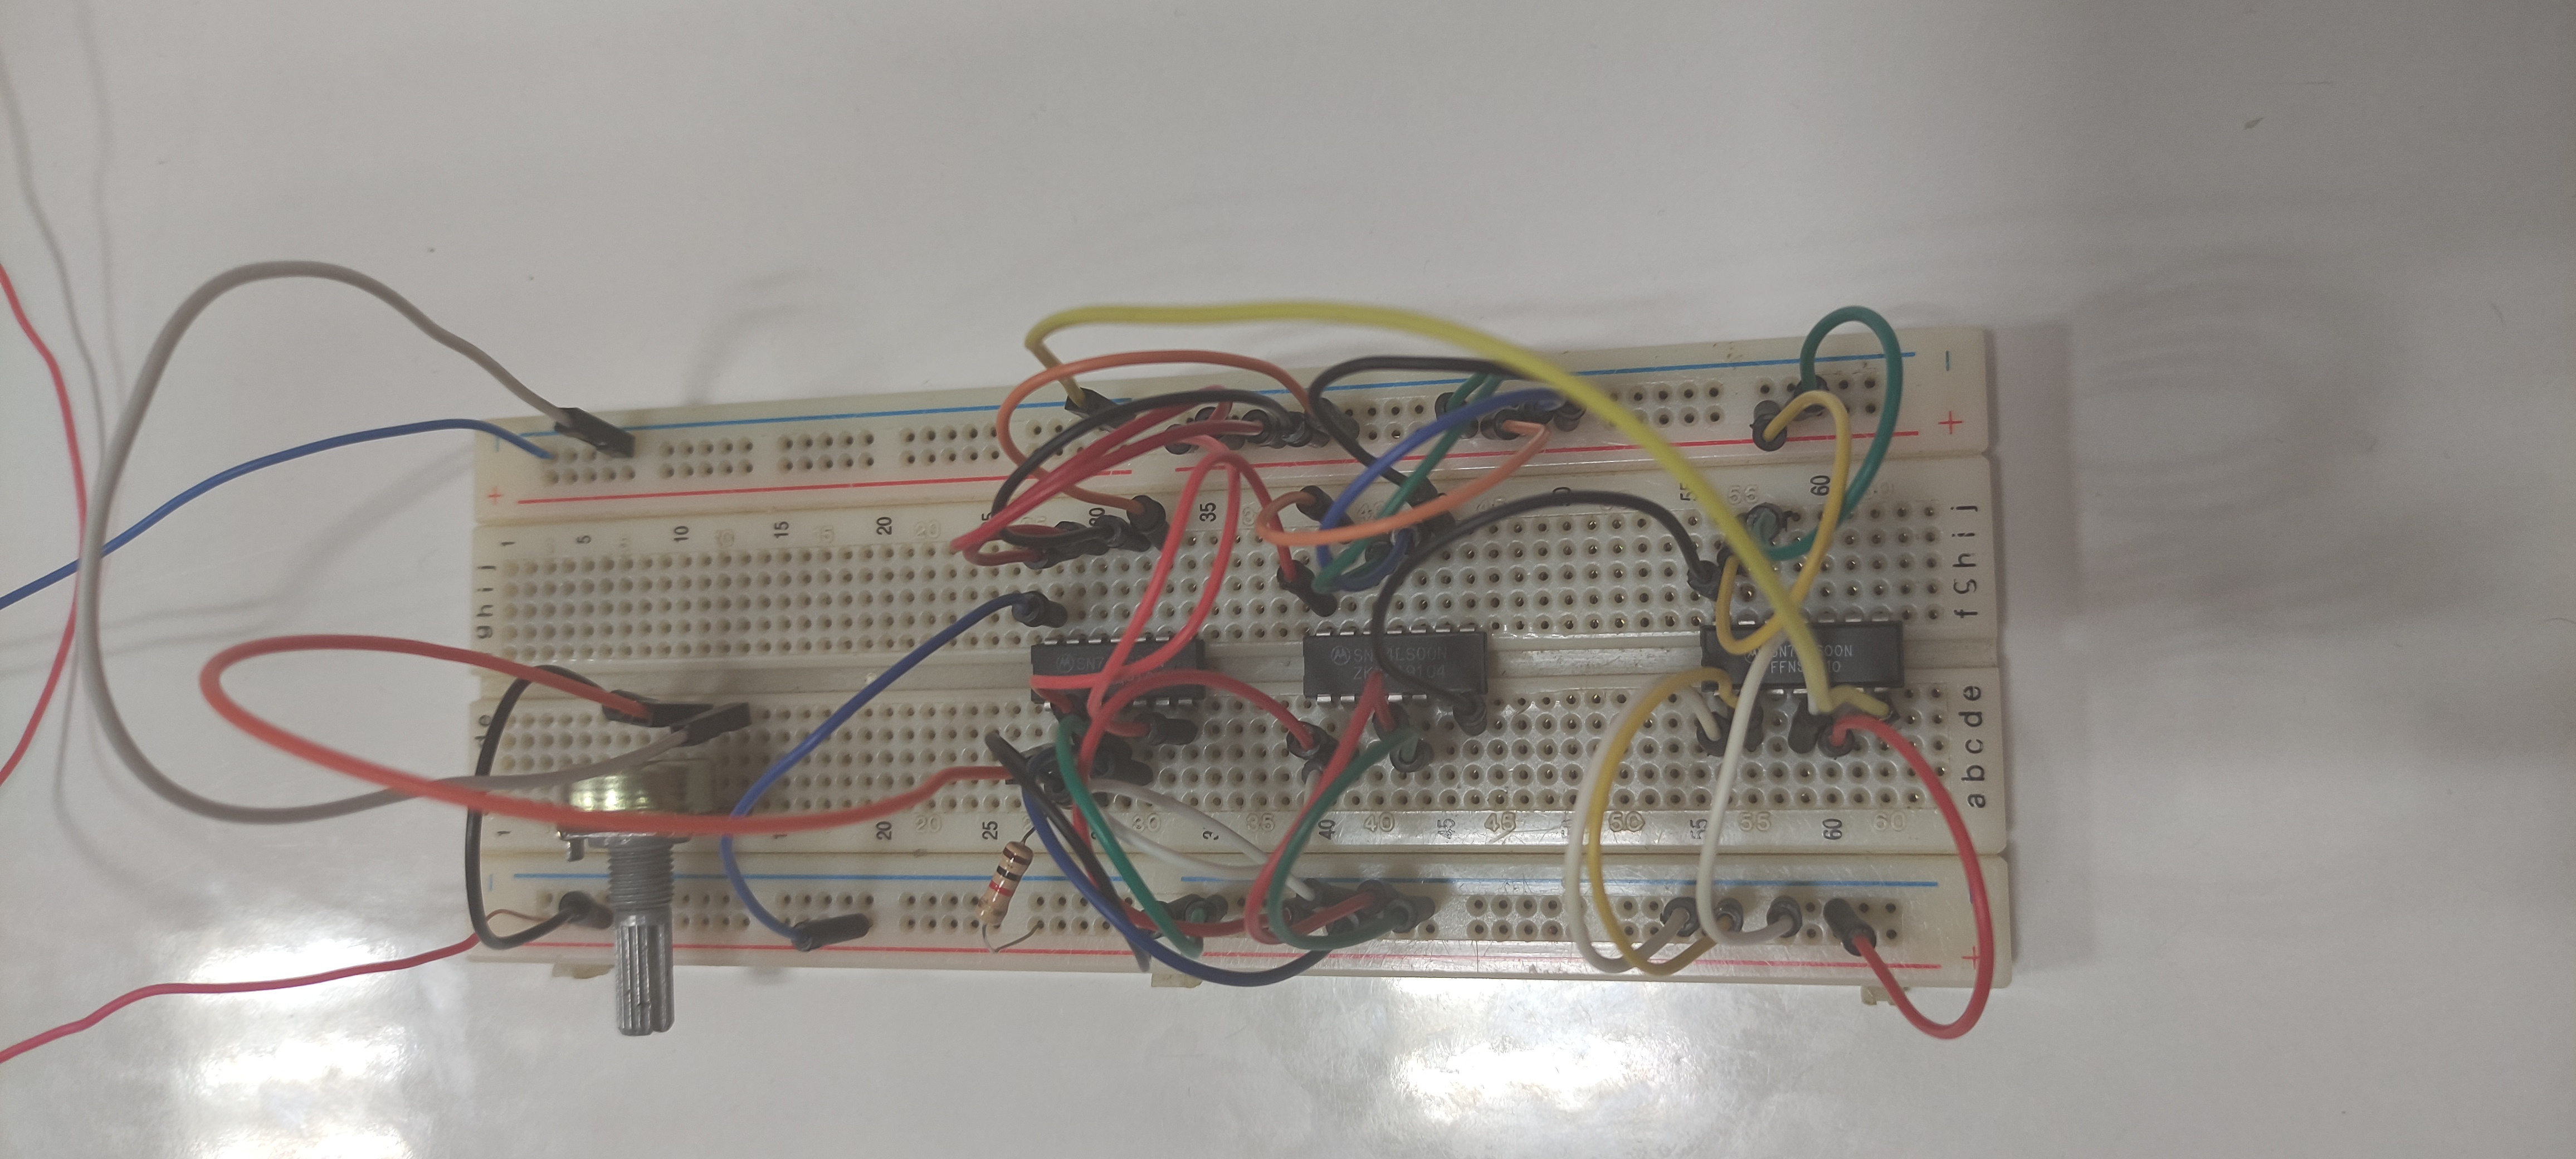
\includegraphics[scale=0.075]{last_madar}‎
				\caption{مدار مرحله آخر آزمایش}
			\end{center}
		\end{figure} 
	
			\begin{figure}[h!]
		\begin{center}
			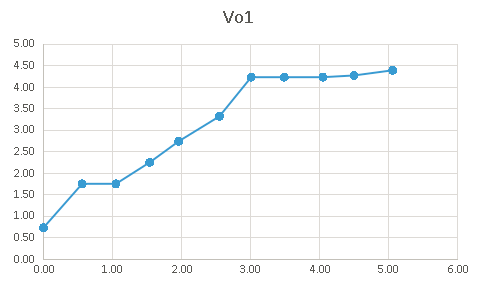
\includegraphics[scale=0.75]{nemoodar3}‎
			\caption{ولتاژ پایه Y1 تراشه اول}
		\end{center}
	\end{figure} 

		\begin{figure}[h!]
		\begin{center}
			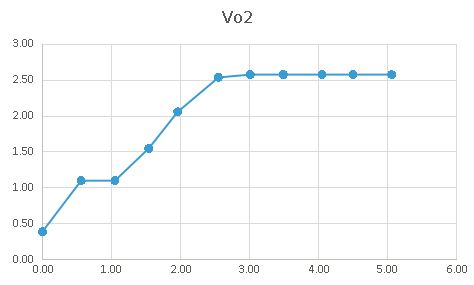
\includegraphics[scale=0.75]{nemoodar4}‎
			\caption{ولتاژ پایه Y1 تراشه دوم}
		\end{center}
	\end{figure} 
	
			\begin{figure}[h!]
		\begin{center}
			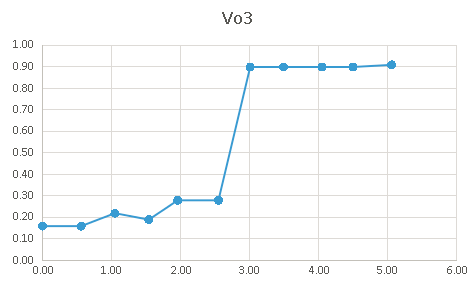
\includegraphics[scale=0.75]{nemoodar5}‎
			\caption{ولتاژ پایه Y1 تراشه سوم}
		\end{center}
	\end{figure} 

	\newpage
	\item
	\subsection*{مشاهدات}
	همانطور که نمودار خروجی تراشه سوم نشان میدهد ، مقدار ولتاژ خروجی در مرز ولتاژ Low تراشه قرار دارد (مطابق دیتاشیت این تراشه ، ولتاژ Low حدود هشت دهم ولت است). البته خروجی منطقی مدار هنوز 1 است ولی با افزایش تعداد گیت ها به بیشتر از 10 گیت ، افت ولتاژ بیشتری رخ داده و پدیده Fan-out رخ میدهد که در نتیجه آن خروجی منطقی مدار 0 خواهد شد که مخالف انتظار است.
	
	\begin{figure}[h!]
		\begin{center}
			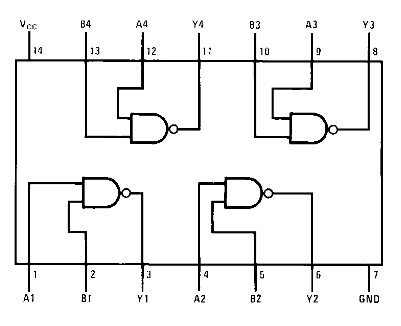
\includegraphics[scale=0.75]{DM74SL00_connection_diagram}‎
			\caption{دیاگرام اتصالات تراشه 7400}
		\end{center}
	\end{figure} 
	
	\end{itemize}
	
\end{document}









